\thispagestyle{thachthuctoanhocnone}
\pagestyle{thachthuctoanhoc}
\everymath{\color{thachthuctoanhoc}}
\graphicspath{{../thachthuctoanhoc/pic/}}
\begingroup
\AddToShipoutPicture*{\put(0,616){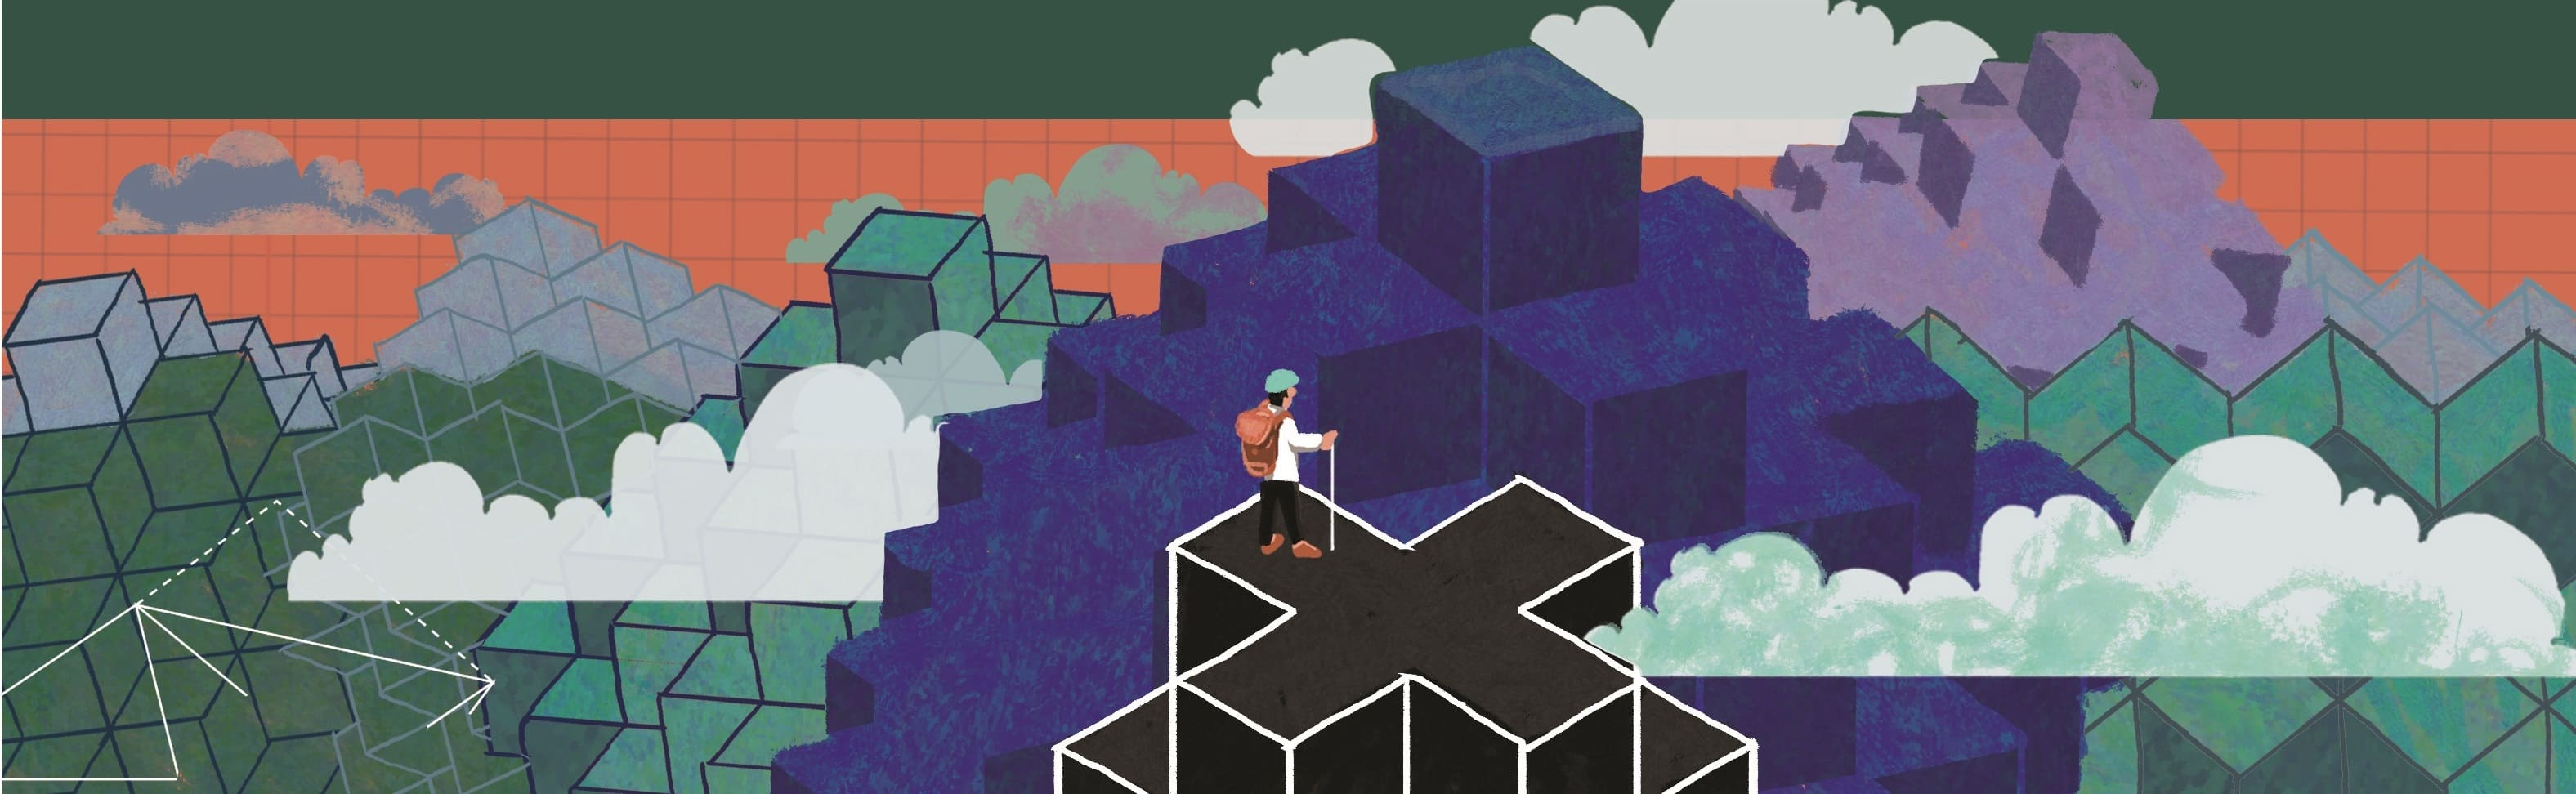
\includegraphics[width=19.3cm]{../thachthuctoanhoc/bannerthachthuc}}}
\centering
\vspace*{4cm}
\endgroup
\vspace*{-8pt}
\begin{tBox}
	\begin{itemize}[leftmargin = 13pt, itemsep = 1.0pt] 
		\item Mỗi bài toán đề xuất (kèm theo lời giải) cần được nêu rõ là bài sáng tác hay bài sưu tầm.
%		\item Mỗi bài toán đề xuất (kèm theo lời giải) cần được nêu rõ là bài sáng tác hay bài sưu tầm (nếu là bài sưu tầm, cần ghi rõ nguồn).
		\item Bài giải cho mỗi bài toán cần được trình bày trong một file riêng hoặc
		một tờ giấy riêng.
		\item  Người đề xuất bài toán hoặc gửi bài giải cho các bài toán trong mục ``Thách thức kỳ này" cần ghi rõ họ, đệm, tên và nơi làm việc/học tập, số điện thoại liên hệ. Nếu là học sinh (hoặc sinh viên) cần ghi rõ là học sinh lớp mấy (hoặc sinh viên năm thứ mấy).
		\item Các bài toán trong mục Thách thức kỳ này hướng tới các độc giả là học sinh phổ thông; được phân chia thành các mức độ $B$, $A$, và được sắp xếp theo độ khó tăng dần, theo đánh giá chủ quan của Ban biên tập. Các bài toán mức độ $B$ không đòi hỏi các kiến thức vượt quá chương trình môn Toán cấp THCS; các bài toán mức độ $A$ không đòi hỏi các kiến thức vượt quá chương trình môn Toán cấp THPT.
		\item Cách thức gửi bài toán đề xuất hoặc lời giải: gửi file thu được bằng cách scan, ảnh chụp (rõ nét) của bản viết tay, hoặc được soạn thảo bằng các phần mềm Latex, Word tới \url{bbt@pi.edu.vn} hoặc gửi qua đường bưu điện tới Tòa soạn (xem địa chỉ tại bìa $2$).
		\item Hạn gửi lời giải cho các bài toán P$711$--P$720$: trước ngày $15/7/2023$.
	\end{itemize}
\end{tBox}
\begin{center}
	\vspace*{-5pt}
	\textbf{\color{thachthuctoanhoc}\color{thachthuctoanhoc}\color{thachthuctoanhoc}THÁCH THỨC KỲ NÀY}
	\vspace*{-5pt}
\end{center}
\begin{multicols}{2}
	\setlength{\abovedisplayskip}{4pt}
	\setlength{\belowdisplayskip}{4pt}
	{\color{thachthuctoanhoc}{\usefont{T5}{qag}{b}{n} P711.}}
	(Mức $B$)Bác An có $6$ tấm thẻ $A,$ $B,$ $C,$ $D,$ $E,$ $F$. Bác ghi các số nguyên dương $1,2,3,4,5,6$ lên mỗi tấm thẻ, sao cho mỗi số được ghi trên đúng một thẻ và mỗi thẻ được ghi đúng một số. Biết rằng tổng các số ghi ở tấm thẻ $A,B,C$ bằng $14$ và tổng các số được ghi ở tấm thẻ $A,D,E$ là $12$. Hỏi bác An có bao nhiêu cách ghi số như vậy?
	\vskip 0.3cm
	\hfill	\textit{Nguyễn Tường Thanh, Hải Dương}
	\vskip 0.3cm
	{\color{thachthuctoanhoc}{\usefont{T5}{qag}{b}{n} P712.}}
	(Mức $B$) Tìm tất cả các số nguyên $a$ sao cho $a^2+a+1$ chỉ có ước nguyên tố không vượt quá $5$. 
	\begin{flushright}
		\textit{Hà Duy Hưng, Hà Nội}
	\end{flushright}
	{\color{thachthuctoanhoc}{\usefont{T5}{qag}{b}{n} P713.}}
	(Mức $B$) Xác định tất cả các cặp số thực $(a;b)$ sao cho $a+b$ là số nguyên và $a^3+b^3=2$. 
	\begin{flushright}
		\textit{Nguyễn Đức Tấn, Tp. Hồ Chí Minh}
	\end{flushright}
	{\color{thachthuctoanhoc}{\usefont{T5}{qag}{b}{n} P714.}}
	(Mức $B$) Cho $2023$ số nguyên dương $a_1,$ $a_2,$ $\ldots,$ $a_{2023}$ thỏa mãn
	\begin{align*}
		\frac{1}{a_1^2}+\frac{1}{a_2^2}+\cdots+\frac{1}{a_{2023}^2}\ge 33.
	\end{align*}
	Chứng minh rằng, trong $2023$ số đó, luôn tìm được ít nhất $21$ số bằng nhau.  
	\begin{flushright}
		\textit{Nguyễn Văn Quý, Hà Nội}
	\end{flushright}
	{\color{thachthuctoanhoc}{\usefont{T5}{qag}{b}{n} P715.}}
	(Mức $B$) Cho tam giác không cân $ABC$ nội tiếp đường tròn $(O)$, có $M$ là trung điểm $BC$. Đường tròn ngoại tiếp tam giác $AMO$ cắt đường tròn $(O)$ tại điểm thứ hai $D$. Đường thẳng $AM$ cắt $(O)$  tại điểm thứ hai $E$. Chứng minh rằng $DE\| BC$. 
	\begin{center}
		\definecolor{qqqqff}{rgb}{0,0,1}
		\definecolor{qqqqffa}{rgb}{1,1,1}
		\definecolor{cqcqcq}{rgb}{0.7529411764705882,0.7529411764705882,0.7529411764705882}
		\begin{tikzpicture}[thachthuctoanhoc,scale=0.6]
			\draw  (-3.26,4.44)-- (-5.22,-1.8);
			\draw  (-5.22,-1.8)-- (2.16,-1.8);
			\draw  (2.16,-1.8)-- (-3.26,4.44);
			\draw  (-1.53,0.4687820512820516) circle (4.331682351721972cm);
			\draw  (-2.0917832603951787,-3.826316499922491)-- (-0.9682167396048218,-3.8263164999224912);
			\draw  (-3.26,4.44)-- (-0.9682167396048218,-3.8263164999224912);
			\draw [shift={(-9.556965317919069,-0.665608974358972)},dash pattern=on 1pt off 1.6pt]  plot[domain=-0.40050890991965815:0.6812945286306901,variable=\t]({1*8.106726541220599*cos(\t r)+0*8.106726541220599*sin(\t r)},{0*8.106726541220599*cos(\t r)+1*8.106726541220599*sin(\t r)});
			\draw [fill=white] (-3.26,4.44) circle (1.6pt);
			\draw (-3.26,4.93) node {$A$};
			\draw [fill=white] (-5.22,-1.8) circle (1.6pt);
			\draw (-5.52,-2.05) node {$B$};
			\draw [fill=white] (2.16,-1.8) circle (1.6pt);
			\draw (2.4,-2.05) node {$C$};
			\draw [fill=white] (-1.53,0.4687820512820516) circle (1.6pt);
			\draw (-1.28,0.71) node {$O$};
			\draw [fill=white] (-1.53,-1.8) circle (1.6pt);
			\draw (-0.8,-2.2) node {$M$};
			\draw [fill=white] (-2.0917832603951787,-3.826316499922491) circle (1.6pt);
			\draw (-2.04,-4.4) node {$D$};
			\draw [fill=white] (-0.9682167396048218,-3.8263164999224912) circle (1.6pt);
			\draw (-1.12,-4.4) node {$E$};
		\end{tikzpicture}
	\end{center}
	\begin{flushright}
		\textit{Bằng Linh, Phú Thọ (st)}
	\end{flushright}
	{\color{thachthuctoanhoc}{\usefont{T5}{qag}{b}{n} P716.}}
	(Mức $B$) Trong một lớp học có $33$ học sinh. Mỗi bạn viết lên bảng số người trong lớp có cùng tên với mình và viết lên bảng số người có cùng họ với mình. Sau khi tất cả học sinh hoàn thành việc viết số, thì trên bảng các số $0,1,2,\ldots,10$ đều xuất hiện ít nhất một lần. Hỏi số $6$ xuất hiện bao nhiêu lần?
	\begin{flushright}
		\textit{Tô Trung Hiếu, Nghệ An (st)}
	\end{flushright}
	{\color{thachthuctoanhoc}{\usefont{T5}{qag}{b}{n} P717.}}
	(Mức $A$) Chứng minh rằng, với mọi bộ ba số thực $(a;b;c)$ thoả mãn  $ac\ne0$ và $b^2\ge4ac$, ta có
	\begin{align*}
		(a-b)^4+(b-c)^4+(c-a)^4 \ge \dfrac{81}{128}c^4.
	\end{align*}
	\begin{flushright}
		\textit{Nguyễn Văn Long, Vĩnh Phúc}
	\end{flushright}
	{\color{thachthuctoanhoc}{\usefont{T5}{qag}{b}{n} P718.}}
	(Mức $A$) Cho tam giác $ABC$ và $P$ là một điểm cố định nằm trong tam giác đó. Một đường thẳng $d$ quay quanh điểm $P$, cắt các đường thẳng $BC,CA,AB$ tương ứng tại các điểm $D,E,F$. Gọi $Q$ là giao điểm thứ hai của hai đường tròn $(ADE)$ và $(APF)$. Chứng minh rằng, $Q$ luôn thuộc một đường tròn cố định.  
	\begin{center}
		\definecolor{ffqqqq}{rgb}{1,0,0}
		\definecolor{qqqqff}{rgb}{0,0,1}
		\definecolor{qqqqffa}{rgb}{1,1,1}
		\begin{tikzpicture}[thachthuctoanhoc, scale=0.7]
			\draw  (-4.76,5.36)-- (-6.22,-0.5);
			\draw  (-6.22,-0.5)-- (0.2,-0.5);
			\draw  (0.2,-0.5)-- (-4.76,5.36);
			\draw [color=ffqqqq] (-5.222691037714135,1.894862071043978) circle (3.4958924272738447cm);
			\draw  (-5.750222132850728,2.8374132314498297) circle (2.709978575054024cm);
			\draw  (-7.76943396226415,-0.5)-- (-1.7287290671233002,1.7787000672061575);
			\draw  (-7.76943396226415,-0.5)-- (-6.22,-0.5);
			\draw [fill=white] (-4.76,5.36) circle (1.6pt);
			\draw (-4.76,5.73) node {$A$};
			\draw [fill=white] (-6.22,-0.5) circle (1.6pt);
			\draw (-6.36,-0.87) node {$B$};
			\draw [fill=white] (0.2,-0.5) circle (1.6pt);
			\draw (0.26,-0.81) node {$C$};
			\draw [fill=white] (-3.74,1.02) circle (1.6pt);
			\draw (-3.5,0.65) node {$P$};
			\draw [fill=white] (-7.76943396226415,-0.5) circle (1.6pt);
			\draw (-8.1,-0.73) node {$D$};
			\draw [fill=white] (-1.7287290671233002,1.7787000672061575) circle (1.6pt);
			\draw (-1.34,1.95) node {$E$};
			\draw [fill=white] (-6.059271801059053,0.14511455191366746) circle (1.6pt);
			\draw (-6.3,0.5) node {$F$};
			\draw [fill=white] (-8.418223065252786,3.3125499506724045) circle (1.6pt);
			\draw (-8.82,3.53) node {$Q$};
		\end{tikzpicture}
	\end{center}
	\begin{flushright}
		\textit{Phạm Vĩnh Minh, Đồng Tháp}
	\end{flushright}
	{\color{thachthuctoanhoc}{\usefont{T5}{qag}{b}{n} P719.}}
	(Mức $A$) Cho $S$ là một tập hữu hạn các số nguyên lớn hơn $1$ thoả mãn: với mỗi số nguyên dương $n$, tồn tại $x\in S$ sao cho  hoặc $x,n$ nguyên tố cùng nhau, hoặc $n$ chia hết cho $x$.  Chứng minh rằng, tồn tại $x,y\in S$ (có thể trùng nhau) sao cho $\gcd(x,y)$ là một số nguyên tố. 
	\begin{flushright}
		\textit{Bằng Linh, Phú Thọ (st)}
	\end{flushright}
	{\color{thachthuctoanhoc}{\usefont{T5}{qag}{b}{n} P720.}}
	(Mức $A$) Trong một thành phố, có $1334$ căn nhà. Mỗi dịp Noel, ông già Noel sẽ đến thăm các căn nhà đó theo thứ tự tùy ý. Chứng minh rằng, trong $3$ năm liên tiếp ta luôn tìm được $12$ căn nhà được ông già Noel đến thăm theo cùng một thứ tự như nhau (theo thời gian trước -- sau) ở $2$ năm trong số $3$ năm đó. 
	\begin{flushright}
		\textit{Trương Bảo Nam, Hà Nội}
	\end{flushright}
	\textbf{\color{thachthuctoanhoc}ĐÍNH CHÍNH:}
	Trong phát biểu của bài toán {\color{thachthuctoanhoc}{\usefont{T5}{qag}{b}{n} P720}} tập $7$ số $5$, công thức của $a$ bị thiếu số $x$, công thức đúng là:
	\begin{align*}
		a=\left\lfloor x+\dfrac12\right\rfloor+\left\lfloor\sqrt{2}x\right\rfloor
	\end{align*} thành thật cáo lỗi cùng bạn đọc.
\end{multicols}
\centerline{{\large{\textbf{\color{thachthuctoanhoc}GIẢI BÀI KỲ TRƯỚC}}}}
\vspace*{-5pt}
\begin{multicols}{2}
	\setlength{\abovedisplayskip}{4pt}
	\setlength{\belowdisplayskip}{4pt}
	{\color{thachthuctoanhoc}{\usefont{T5}{qag}{b}{n} P681.}}
	(Mức $B$) Một số có bốn chữ số $\overline{a b c d}$ được gọi là số ``zig zag", nếu $a, b, c, d$ đôi một khác nhau, và $a<b, b>c, c<d$ (chẳng hạn, $1204$ là số ``zig zag"). Hỏi có bao nhiêu số ``zig zag" có chữ số hàng nghìn là $7$?
	\vskip 0.05cm
	\textbf{\color{thachthuctoanhoc}Lời giải} (\textit{phỏng theo cách giải của bạn Trần Hữu Dương, lớp $11$ Toán $1$, trường THPT chuyên Hưng Yên, tỉnh Hưng Yên})\textbf{\color{thachthuctoanhoc}.}
	Vì $a = 7$ và $b > a$ (giả thiết), nên $b \in \{8; 9\}$. \hfill ($1$)
	\vskip 0.05cm
	Vì $b, d$ cùng lớn hơn $c$, và $b$, $c$, $d$ đôi một khác nhau (giả thiết), nên
	\begin{align*}
		c \le \max\{b, d\} - 2 \le 9 - 2 = 7.
	\end{align*}
	Từ đó, do $c \ne a = 7$, suy ra $c \in \{0; 1; 2; 3;$ $4; 5; 6\}$. \hfill($2$)
	\vskip 0.05cm
	Rõ ràng, với mỗi $b$ thỏa mãn ($1$), tất cả $c$ thỏa mãn ($2$) đều đáp ứng yêu cầu $c < b$.
	\vskip 0.05cm
	Tiếp theo, dễ thấy, với mỗi $c = k \in \{0; 1; 2;$ $3; 4; 5; 6\}$, có $7 - k$ giá trị của $d$ thỏa mãn yêu cầu $d > c$, là: $k \!+\! 1, k \!+\! 2, \ldots, 9$, trừ ra $7$ và $b$.
	\vskip 0.05cm
	Vì vậy, với $a = 7$, số bộ ($b, c, d$) thỏa mãn $a < b, b > c, c < d$ là:
	\begin{align*}
		2(7 + 6 + 5 + 4 + 3 + 2 + 1) = 56.
	\end{align*}
	Vậy, có $56$ số ``zig zag" có chữ số hàng nghìn là $7$.
	\vskip 0.05cm
	\textbf{\color{thachthuctoanhoc}Bình luận và Nhận xét}
	\vskip 0.05cm	
	Trong số các lời giải Tạp chí đã nhận được từ bạn đọc, rất tiếc, có:
	\vskip 0.05cm
	-- Một lời giải sai, do người giải bài không lưu ý tới ràng buộc ``$a$, $b$, $c$, $d$ đôi một khác nhau";
	\vskip 0.05cm
	-- Một lời giải không được chấp nhận là lời giải hoàn chỉnh, do người giải bài chỉ nêu ra số các cặp $(c, d)$ thỏa mãn yêu cầu của bài toán, mà không có bất cứ lý giải nào.
	\begin{flushright}
		\textbf{\color{thachthuctoanhoc}Lê Huy}
	\end{flushright}
	{\color{thachthuctoanhoc}{\usefont{T5}{qag}{b}{n} P682.}}
	(Mức $B$) Cho $100$ số hữu tỷ $a_1,a_2,\ldots,a_{100}$ thoả mãn $a_1+a_4=4$ và
	\begin{align*}
		\dfrac{a_1+a_2}1=\dfrac{a_2+a_3}2=\cdots=\dfrac{a_{100}+a_1}{100}.
	\end{align*}
	Tính tổng $a_1+ a_2 +\cdots+a_{100}$. 
	
	{\color{thachthuctoanhoc}{\usefont{T5}{qag}{b}{n} P683.}}
	(Mức $B$) Cho tam giác $ABC$ có $\angle BAC\ne90^\circ$ và nội tiếp $(O)$. Gọi $M$ là trung điểm của cạnh $BC$. Đường tròn đi qua $A$ và tiếp xúc với $BC$ tại $B$, cắt $AM$ tại điểm thứ hai $D$ (khác $A$). Các đường thẳng $BD$, $CD$ tương ứng cắt $(O)$ tại các điểm thứ hai $E$, $F$. Chứng minh rằng $AM$ là phân giác của góc $\angle EAF$. 
	\vskip 0.05cm
	\textbf{\color{thachthuctoanhoc}Lời giải} (\textit{của người chấm bài})\textbf{\color{thachthuctoanhoc}.}
	\begin{figure}[H]
		\vspace*{-5pt}
		\centering
		\captionsetup{labelformat= empty, justification=centering}
		\definecolor{qqwuqq}{rgb}{0.,0.39215686274509803,0.}
		\definecolor{uuuuuu}{rgb}{0.26666666666666666,0.26666666666666666,0.26666666666666666}
		\definecolor{qqqqff}{rgb}{0.,0.,1.}
		\begin{tikzpicture}[thachthuctoanhoc,scale=0.6]
			\draw [shift={(-1.,-1.)},,pattern color=qqwuqq,fill=qqwuqq,fill opacity=0.10000000149011612] (0,0) -- (0.:0.4) arc (0.:36.027373385103616:0.4) -- cycle;
			\draw [shift={(0.,5.)},,pattern color=qqwuqq,fill=qqwuqq,fill opacity=0.10000000149011612] (0,0) -- (-99.46232220802563:0.4) arc (-99.46232220802563:-63.43494882292201:0.4) -- cycle;
			\draw [shift={(0.,5.)},,pattern color=qqwuqq,fill=qqwuqq,fill opacity=0.10000000149011612] (0,0) -- (-63.43494882292201:0.6) arc (-63.43494882292201:-40.601294645004465:0.6) -- cycle;
			\draw [shift={(7.,-1.)},,pattern color=qqwuqq,fill=qqwuqq,fill opacity=0.10000000149011612] (0,0) -- (157.16634582208246:0.6) arc (157.16634582208246:180.:0.6) -- cycle;
			\draw [shift={(0.,5.)},,pattern color=qqwuqq,fill=qqwuqq,fill opacity=0.10000000149011612] (0,0) -- (-40.60129464500447:0.4) arc (-40.60129464500447:-4.573921259900855:0.4) -- cycle;
			\draw [shift={(0.,5.)},,pattern color=qqwuqq,fill=qqwuqq,fill opacity=0.10000000149011612] (0,0) -- (-122.29597638594316:0.6) arc (-122.29597638594316:-99.46232220802563:0.6) -- cycle;
			\draw [] (0.,5.)-- (-1.,-1.);
			\draw [] (7.,-1.)-- (0.,5.);
			\draw [] (3.,1.4166666666666667) circle (4.673358297603317cm);
			\draw [] (-1.,2.0833333333333335) circle (3.0833333333333335cm);
			\draw [] (0.,5.)-- (3.,-1.);
			\draw [] (-1.52392156862745,2.589019607843137)-- (0.,5.);
			\draw [] (0.,5.)-- (6.531531531531531,4.477477477477478);
			\draw (-0.4,5.9) node[anchor=north west] {$A$};
			\draw (-1.7,-1) node[anchor=north west] {$B$};
			\draw (7.,-0.76) node[anchor=north west] {$C$};
			\draw (2.56,-1) node[anchor=north west] {$M$};
			\draw (2.92,1.6) node[anchor=north west] {$O$};
			\draw (1.68,1.16) node[anchor=north west] {$D$};
			\draw (6.52,5.12) node[anchor=north west] {$E$};
			\draw (-2.3,3.1) node[anchor=north west] {$F$};
			\draw [] (6.531531531531531,4.477477477477478)-- (-1.,-1.);
			\draw [] (-1.52392156862745,2.589019607843137)-- (7.,-1.);
			\draw [shift={(0.,5.)},,color=qqwuqq] (-63.43494882292201:0.6) arc (-63.43494882292201:-40.601294645004465:0.6);
			\draw [shift={(0.,5.)},,color=qqwuqq] (-63.43494882292201:0.5) arc (-63.43494882292201:-40.601294645004465:0.5);
			\draw [shift={(7.,-1.)},,color=qqwuqq] (157.16634582208246:0.6) arc (157.16634582208246:180.:0.6);
			\draw [shift={(7.,-1.)},,color=qqwuqq] (157.16634582208246:0.5) arc (157.16634582208246:180.:0.5);
			\draw [] (-1.,-1.)-- (-1.52392156862745,2.589019607843137);
			\draw [shift={(0.,5.)},,color=qqwuqq] (-122.29597638594316:0.6) arc (-122.29597638594316:-99.46232220802563:0.6);
			\draw [shift={(0.,5.)},,color=qqwuqq] (-122.29597638594316:0.5) arc (-122.29597638594316:-99.46232220802563:0.5);
			\draw [] (3.,-1.)-- (-1.,-1.);
			\draw [] (1.035,-1.09) -- (1.035,-0.91);
			\draw [] (0.965,-1.09) -- (0.965,-0.91);
			\draw [] (3.,-1.)-- (7.,-1.);
			\draw [] (4.965,-0.91) -- (4.965,-1.09);
			\draw [] (5.035,-0.91) -- (5.035,-1.09);
				\draw [fill=white] (0.,5.) circle (1.5pt);
				\draw [fill=white] (-1.,-1.) circle (1.5pt);
				\draw [fill=white] (7.,-1.) circle (1.5pt);
				\draw [fill=white] (3.,-1.) circle (1.5pt);
				\draw [fill=white] (3.,1.4166666666666667) circle (1.5pt);
				\draw [fill=white] (0.,5.) circle (1.5pt);
				\draw [fill=white] (1.9333333333333331,1.1333333333333335) circle (1.5pt);
				\draw [fill=white] (7.,-1.) circle (1.5pt);
				\draw [fill=white] (-1.52392156862745,2.589019607843137) circle (1.5pt);
				\draw [fill=white] (-1.,-1.) circle (1.5pt);
				\draw [fill=white] (6.531531531531531,4.477477477477478) circle (1.5pt);
		\end{tikzpicture}
		\caption{\small\textit{\color{thachthuctoanhoc}Hình $1$}}
		\vspace*{-10pt}
	\end{figure}
	Do $MB$ tiếp xúc với đường tròn $(ABD)$ tại $B$, nên
	\begin{align*}
		\angle MAB = \angle MBD.
	\end{align*}
	Suy ra, $\Delta MAB \sim \Delta MBD$. Do đó
	\begin{align*}
		\frac{{MA}}{{MB}} = \frac{{MB}}{{MD}}.
	\end{align*}
	Từ đó, do $M$ là trung điểm $BC$ (giả thiết), ta được:
	\begin{align*}
		M{C^2} = M{B^2} = MD \cdot MA.
	\end{align*}
	Suy ra, $\dfrac{{MA}}{{MC}} = \dfrac{{MC}}{{MD}}$.  Do đó, $\Delta MAC \sim \Delta MCD$. Vì vậy
	\begin{align*}
		\angle MAC = \angle MCD. \tag{$2$}
	\end{align*}
	Do $\angle BAC \ne {90^{\circ}}$  (giả thiết), nên có thể xảy ra hai trường hợp sau:
	\vskip 0.05cm
	$\diamond$ \textit{Trường hợp $1$: $\angle BAC$ là góc nhọn.}
	\vskip 0.05cm
	Khi đó, điểm $D$ nằm giữa hai điểm $A$, $M$; do đó, $E$ nằm trên cung $AC$ không chứa $B$, và $F$ nằm trên cung $AB$ không chứa $C$, của đường tròn $(O)$. (Xem Hình $1$).
	\vskip 0.05cm
	Vì thế, $ABCE$ và $ACBF$ là các tứ giác lồi nội tiếp; tia $AB$ nằm giữa hai tia $AF$, $AM$, và tia $AC$ nằm giữa hai tia $AM$, $AE$. Do đó
	\begin{align*}
		&\angle CAE = \angle CBE = \angle MBD, \tag{$3$}\\
		&\angle FAB = \angle BCF = \angle MCD, \tag{$4$}\\
		&\angle FAM = \angle FAB + \angle BAM,\tag{$5$}\\
		&\angle MAE = \angle MAC + \angle CAE.\tag{$6$}
	\end{align*}
	Từ ($3$) và ($1$), suy ra $\angle CAE = \angle MAB.$  \hfill ($7$)
	\vskip 0.05cm
	Từ ($4$) và ($2$), suy ra $\angle FAB = \angle MAC.$ \hfill ($8$)
	\vskip 0.05cm
	Từ ($5$), ($6$), ($7$), ($8$), suy ra $\angle FAM = \angle MAE$.  Vì thế, $AM$ là phân giác của góc $EAF$.
	\vskip 0.05cm
	$\diamond$ \textit{Trường hợp $2$: $\angle BAC$  là góc tù.}
	\vskip 0.05cm
	Trong trường hợp này, điểm $A$ nằm giữa hai điểm $D$, $M$; do đó, $E$ nằm trên cung $AC$ chứa $B$, và $F$ nằm trên cung $AB$ chứa $C$, của đường tròn $(O)$.
	\vskip 0.05cm
	Vì thế, có thể xảy ra các khả năng sau:
	\vskip 0.05cm
	-- \textit{Khả năng} $2.1$: $E$ nằm trên cung $AB$ không chứa $C$, và $F$ nằm trên cung $AC$ không chứa $B$, của đường tròn $(O)$.
	\vskip 0.05cm
	-- \textit{Khả năng} $2.2$: $E$ nằm trên cung $BC$ không chứa $A$, và $F$ nằm trên cung $AC$ không chứa $B$, của đường tròn $(O)$.
	\vskip 0.05cm
	-- \textit{Khả năng} $2.3$: $E$ nằm trên cung $AB$ không chứa $C$, và $F$ nằm trên cung $BC$ không chứa $A$, của đường tròn $(O)$.
	\vskip 0.05cm
	Dưới đây, ta sẽ xét khả năng $2.1$ (xem Hình $2$); hai khả năng còn lại ($2.2$ và $2.3$) được xét theo cách tương tự.
	\begin{figure}[H]
		\vspace*{-5pt}
		\centering
		\captionsetup{labelformat= empty, justification=centering}
		\definecolor{qqwuqq}{rgb}{0.,0.39215686274509803,0.}
		\definecolor{uuuuuu}{rgb}{0.26666666666666666,0.26666666666666666,0.26666666666666666}
		\definecolor{xdxdff}{rgb}{0.49019607843137253,0.49019607843137253,1.}
		\definecolor{qqqqff}{rgb}{0.,0.,1.}
		\begin{tikzpicture}[thachthuctoanhoc,scale=0.6]
			\draw [shift={(1.8267105859605084,5.824054386499082)},,pattern color=qqwuqq,fill=qqwuqq,fill opacity=0.10000000149011612] (0,0) -- (-133.48963894565472:0.4) arc (-133.48963894565472:-67.65164216337305:0.4) -- cycle;
			\draw [shift={(-0.8805700005813275,2.9701425001453328)},,pattern color=qqwuqq,fill=qqwuqq,fill opacity=0.10000000149011612] (0,0) -- (0.:0.4) arc (0.:65.83799678228164:0.4) -- cycle;
			\draw [shift={(6.8805700005813275,2.970142500145332)},,pattern color=qqwuqq,fill=qqwuqq,fill opacity=0.10000000149011612] (0,0) -- (141.80175331435518:0.6) arc (141.80175331435518:180.:0.6) -- cycle;
			\draw [shift={(1.8267105859605084,5.824054386499082)},,pattern color=qqwuqq,fill=qqwuqq,fill opacity=0.10000000149011612] (0,0) -- (-67.65164216337305:0.6) arc (-67.65164216337305:-29.453395477728233:0.6) -- cycle;
			\draw [] (3.,2.) circle (4.cm);
			\draw [] (-0.8805700005813275,2.9701425001453328)-- (6.8805700005813275,2.970142500145332);
			\draw [] (6.8805700005813275,2.970142500145332)-- (1.8267105859605084,5.824054386499082);
			\draw [] (1.8267105859605084,5.824054386499082)-- (-0.8805700005813275,2.9701425001453328);
			\draw [] (-0.8805700005813272,5.681189975599776) circle (2.711047475454443cm);
			\draw [] (-0.30487452631651313,4.253398403590497)-- (1.8267105859605084,5.824054386499082);
			\draw [] (1.8267105859605084,5.824054386499082)-- (3.0302104433382717,5.999885914512225);
			\draw (1.7,6.69) node[anchor=north west] {$A$};
			\draw (-1.69,3.12) node[anchor=north west] {$B$};
			\draw (6.92,3.2) node[anchor=north west] {$C$};
			\draw (2.78,4) node[anchor=north west] {$M$};
			\draw (1.06,8.22) node[anchor=north west] {$D$};
			\draw (-1.3,4.94) node[anchor=north west] {$E$};
			\draw (2.9,6.8) node[anchor=north west] {$F$};
			\draw [shift={(6.8805700005813275,2.970142500145332)},,color=qqwuqq] (141.80175331435518:0.6) arc (141.80175331435518:180.:0.6);
			\draw [shift={(6.8805700005813275,2.970142500145332)},,color=qqwuqq] (141.80175331435518:0.5) arc (141.80175331435518:180.:0.5);
			\draw [shift={(1.8267105859605084,5.824054386499082)},,color=qqwuqq] (-67.65164216337305:0.6) arc (-67.65164216337305:-29.453395477728233:0.6);
			\draw [shift={(1.8267105859605084,5.824054386499082)},,color=qqwuqq] (-67.65164216337305:0.5) arc (-67.65164216337305:-29.453395477728233:0.5);
			\draw [] (1.1443570196456636,7.483812780548872)-- (6.8805700005813275,2.970142500145332);
			\draw [] (3.,2.9701425001453323)-- (1.8267105859605084,5.824054386499082);
			\draw [] (-0.8805700005813275,2.9701425001453328)-- (1.1443570196456636,7.483812780548872);
			\draw (2.76,2.14) node[anchor=north west] {$O$};
			\draw [] (1.8267105859605084,5.824054386499082)-- (1.1443570196456636,7.483812780548872);
			\begin{scriptsize}
				\draw [fill=white] (3.,2.) circle (1.5pt);
				\draw [fill=white] (-0.8805700005813275,2.9701425001453328) circle (1.5pt);
				\draw [fill=white] (6.8805700005813275,2.970142500145332) circle (1.5pt);
				\draw [fill=white] (1.8267105859605084,5.824054386499082) circle (1.5pt);
				\draw [fill=white] (3.,2.9701425001453323) circle (1.5pt);
				\draw [fill=white] (1.1443570196456636,7.483812780548872) circle (1.5pt);
				\draw [fill=white] (1.8267105859605075,5.824054386499084) circle (1.5pt);
				\draw [fill=white] (6.8805700005813275,2.970142500145332) circle (1.5pt);
				\draw [fill=white] (3.0302104433382717,5.999885914512225) circle (1.5pt);
				\draw [fill=white] (-0.8805700005813275,2.9701425001453328) circle (1.5pt);
				\draw [fill=white] (-0.30487452631651313,4.253398403590497) circle (1.5pt);
			\end{scriptsize}
		\end{tikzpicture}
		\caption{\small\textit{\color{thachthuctoanhoc}}}
		\vspace*{-10pt}
	\end{figure}
	Trong trường hợp này, $AEBC$ và $AFCB$ là các tứ giác lồi nội tiếp; tia $AM$ nằm giữa hai tia $AE$, $AC$, đồng thời nằm giữa hai tia $AB$, $AF$. Do đó
	\begin{align*}
			\angle EAM &= \angle EAC - \angle MAC\\
			&= \left( {{{180}^{\circ}} - \angle EBC} \right) - \angle MAC\\
			&= \left( {{{180}^{\circ}} - \angle MBD} \right) - \angle MAC\\
			&= {180^{\circ}} - \angle MAB - \angle MAC\,\,({\text{do}}(1))\\
			&= {180^{\circ}} - \angle BAC;\tag{$9$}\\
				\angle FAM &= \angle FAB - \angle MAB\\
				&= \left( {{{180}^{\circ}} - \angle BCF} \right) - \angle MAB\\
				&= \left( {{{180}^{\circ}} - \angle MCD} \right) - \angle MAB\\
				&= {180^{\circ}} - \angle MAC - \angle MAB\,\,({\text{do}}(2))\\
				&= {180^{\circ}} - \angle BAC. \tag{$10$}
	\end{align*}
	Từ ($9$) và ($10$) suy ra, $\angle EAM = \angle FAM$.  Vì thế, $AM$ là phân giác của góc $EAF$.
	\vskip 0.05cm
	$\diamond$ Kết quả xét hai trường hợp trên đây cho ta điều phải chứng minh theo yêu cầu đề bài.
	\vskip 0.05cm
	\textbf{\color{thachthuctoanhoc}Bình luận và Nhận xét}
	\vskip 0.05cm
	$\pmb{1.}$ Để tránh việc xét các trường hợp, như ở Lời giải trên, phải sử dụng góc định hướng. Chúng tôi đã không trình bày lời giải theo cách vừa nêu, để các bạn học sinh cấp THCS có thể hiểu lời giải.
	\vskip 0.05cm
	$\pmb{2.}$ Trong số các lời giải Tạp chí đã nhận được từ bạn đọc, lời giải của bạn \textit{Nguyễn Hữu Trí} (lớp $11$A$1$, THPT số $2$ Phù Cát, Bình Định) là lời giải duy nhất đúng và hoàn chỉnh; tất cả các lời giải còn lại chỉ đúng cho trường hợp góc $BAC$ là góc nhọn.
	\begin{flushright}
		\textbf{\color{thachthuctoanhoc}Hạ Vũ Anh}
	\end{flushright}
	{\color{thachthuctoanhoc}{\usefont{T5}{qag}{b}{n} P684.}}
	(Mức $B$) Trong mặt phẳng toạ độ $Oxy$, cho một đường ``trái tim'' như hình dưới đây. Biết rằng, điểm $M(x;y)$ thuộc đường đó khi và chỉ khi $\left(x^2\!+\!y^2\!-\!4\right)^{\!3}\!=\! x^2y^3$. Hỏi có bao nhiêu điểm nguyên thuộc đường đó?  
	\vskip 0.05cm
	({\it Điểm nguyên là điểm có cả hoành độ và tung độ đều là các số nguyên}).
	\begin{figure}[H]
		\centering
		\vspace*{-5pt}
		\captionsetup{labelformat= empty, justification=centering}
		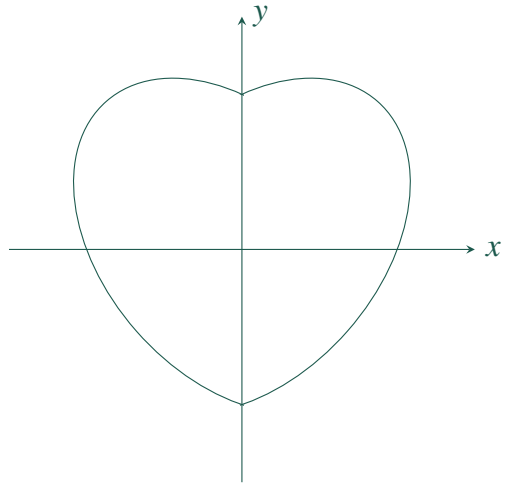
\includegraphics[width=0.8\linewidth]{P1}
	\end{figure}
	\textbf{\color{thachthuctoanhoc}Lời giải} (\textit{dựa theo cách giải của một bạn học sinh lớp $11$ THPT})\textbf{\color{thachthuctoanhoc}.}
	\vskip 0.05cm
	$\bullet$ Giả sử $M(x, y)$ là một điểm nguyên thuộc đường ``trái tim" đã cho trong đề bài. Khi đó, theo giả thiết của bài ra, ta có:
	\begin{align*}
		{\left( {{x^2} + {y^2} - 4} \right)^3} = {x^2}{y^3}. \tag{$1$}
	\end{align*}
	Tiếp theo, ta có:
	\begin{align*}
		(1) &\Leftrightarrow {x^2} + {y^2} - 4 = \sqrt[3]{{{x^2}}} \cdot y\\ &\Leftrightarrow {y^2} - \sqrt[3]{{{x^2}}} \cdot y + {x^2} - 4 = 0.
	\end{align*}
	Do đó, phương trình ẩn $t$ dưới đây là phương trình có nghiệm thực:
	\begin{align*}
		{t^2} - \sqrt[3]{{{x^2}}} \cdot t + {x^2} - 4 = 0.
	\end{align*}
	Suy ra
	\begin{align*}
		\Delta  &= \sqrt[3]{{{x^4}}} - 4{x^2} + 16 \\
		&=  - \sqrt[3]{{{x^4}}}\left( {4\sqrt[3]{{{x^2}}} - 1} \right) + 16 \ge 0. \tag{$2$}
	\end{align*}
	Nhận thấy, nếu $\sqrt[3]{{{x^2}}} \ge 2$  thì
	\begin{align*}
		-\! \sqrt[3]{{{x^4}}}\left( {4\sqrt[3]{{{x^2}}} \!-\! 1} \right) \le  \!-\! {2^2}\left( {4 \cdot 2 \!-\! 1} \right) =  \!-\! 28;
	\end{align*}
	do đó, $\Delta \le - 28 + 16 = -12$, mâu thuẫn với ($2$).
	\vskip 0.05cm
	Vì vậy, $\sqrt[3]{{{x^2}}} < 2$; suy ra, $x^2 < 8$. Mà $x \in \mathbb{Z}$ nên ${x^2} \in \left\{ {0;1;4} \right\}$.
	\vskip 0.05cm 
	-- Với $x^2 = 0$  từ ($1$) ta được $y = \pm 2$.
	\vskip 0.05cm 
	-- Với $x^2 = 1$  từ ($1$) ta được $y (y-1) = 3$,  là điều vô lý, vì $y(y-1)$  là một số chẵn (do  $y \in \mathbb{Z}$).
	\vskip 0.05cm
	-- Với $x^2 = 4$  từ ($1$) ta được $y = 0$.
	\vskip 0.05cm
	Như vậy, nếu điểm nguyên $M(x, y)$ thuộc đường ``trái tim" thì
	\begin{align*}
		\left( {x,y} \right) \!\in\! \left\{\! {\left( {0, \!-\! 2} \right)\!;\!\left( {0,2} \right)\!;\!\left( { \!-\! 2,0} \right)\!;\!\left( {2,0} \right)} \!\right\}. \tag{$3$}
	\end{align*}
	$\bullet$ Ngược lại, bằng cách kiểm tra trực tiếp, dễ thấy, tất cả các điểm nguyên $M(x, y)$, với $(x, y)$ thỏa mãn ($3$), đều thuộc đường ``trái tim".
	\vskip 0.05cm
	$\bullet$ Vậy, có tất cả bốn điểm nguyên thuộc đường ``trái tim" đã cho trong đề bài.
	\vskip 0.05cm
	\textbf{\color{thachthuctoanhoc}Bình luận và Nhận xét}
	\vskip 0.05cm
	Trong số các lời giải Tạp chí đã nhận được từ bạn đọc, chỉ có hai lời giải là lời giải đúng và hoàn chỉnh, tuy cách giải khá dài dòng. Các lời giải còn lại là lời giải không hoàn chỉnh, do có ít nhất một trong các khiếm khuyết sau:
	\vskip 0.05cm
	-- Thiếu phần trình bày cách giải một bất phương trình bậc ba không tầm thường;
	\vskip 0.05cm
	-- Thiếu phần chứng minh các điểm nguyên $M(x, y)$, với $(x, y)$ thỏa mãn ($3$) trong lời giải trên, thuộc đường ``trái tim".
	\begin{flushright}
		\textbf{\color{thachthuctoanhoc}Hà Thanh}
	\end{flushright}
	{\color{thachthuctoanhoc}{\usefont{T5}{qag}{b}{n} P685.}}
	(Mức $B$) Cho $2023$ hình có tổng diện tích lớn hơn $2023$ nằm bên trong một hình vuông diện tích $1$. Chứng minh rằng, $2023$ hình đó có ít nhất một điểm chung.
	\vskip 0.05cm
	{\color{thachthuctoanhoc}{\usefont{T5}{qag}{b}{n} P686.}}
	(Mức $B$) Cho $a,b,c$ là các số thực dương. Chứng minh rằng
	\begin{align*}
		&\dfrac{\sqrt{b c}}{a\!+\!\sqrt{(a\!+\!b)(a\!+\!c)}}+\dfrac{\sqrt{c a}}{b+\sqrt{(b+c)(b+a)}}\\
		&+\dfrac{\sqrt{a b}}{c+\sqrt{(c+a)(c+b)}} \geq 1.
	\end{align*}
	\textbf{\color{thachthuctoanhoc}Lời giải} (\textit{dựa theo tất cả lời giải Tạp chí đã nhận được từ bạn đọc})\textbf{\color{thachthuctoanhoc}.}
	\vskip 0.05cm
	Do $a, b, c > 0$, nên theo bất đẳng thức trung bình cộng -- trung bình nhân cho hai số thực dương, ta có:
	\begin{align*}
			&\frac{{\sqrt {bc} }}{{a + \sqrt {\left( {a + b} \right)\left( {a + c} \right)} }} \\
			= &\frac{{bc}}{{a\sqrt {bc}  + \sqrt {\left( {ac + bc} \right)\left( {ab + bc} \right)} }}\\
			 \ge &\frac{{bc}}{{a \cdot \dfrac{{b + c}}{2} + \dfrac{{\left( {ac + bc} \right) + \left( {ab + bc} \right)}}{2}}}\\
			 = &\frac{{bc}}{{ab + bc + ca}}.
	\end{align*}
	Bằng cách hoàn toàn tương tự, ta cũng chứng minh được:
	\begin{align*}
		&\frac{{\sqrt {ca} }}{{b + \sqrt {\left( {b + c} \right)\left( {b + a} \right)} }} \ge \frac{{ca}}{{ab + bc + ca}}\\
		&\frac{{\sqrt {ab} }}{{c + \sqrt {\left( {c + a} \right)\left( {c + b} \right)} }} \ge \frac{{ab}}{{ab + bc + ca}}.
	\end{align*}
	Cộng ba bất đẳng thức nêu trên, vế theo vế, ta thu được bất đẳng thức cần chứng minh theo yêu cầu đề bài.
	\vskip 0.05cm
	\textbf{\color{thachthuctoanhoc}Bình luận và Nhận xét}
	\vskip 0.05cm
	$\pmb{1.}$ Từ lời giải trên, dễ thấy, dấu đẳng thức, ở bất đẳng thức cần chứng minh của đề bài, xảy ra khi và chỉ khi $a = b = c$.
	\vskip 0.05cm
	$\pmb{2.}$ Tất cả các lời giải Tạp chí đã nhận được từ bạn đọc đều là lời giải đúng và hoàn chỉnh.
	\begin{flushright}
		\textbf{\color{thachthuctoanhoc}Võ Quốc Bá Cẩn}
	\end{flushright}
	{\color{thachthuctoanhoc}{\usefont{T5}{qag}{b}{n} P687.}}
	(Mức $A$) Tìm tất cả các cặp số thực $(p;q)$, sao cho phương trình $x^3-px+q=0$ có ba nghiệm thực phân biệt $a,b,c$  thoả mãn:
	\begin{align*}
		a^2-b=b^2-c=c^2-a.
	\end{align*}
	\textbf{\color{thachthuctoanhoc}Lời giải} (\textit{của người chấm bài})\textbf{\color{thachthuctoanhoc}.}
	\vskip 0.05cm
	$\bullet$ Giả sử $(p, q)$ là cặp số thực thỏa mãn yêu cầu đề bài.
	\vskip 0.05cm
	Khi đó, do phương trình
	\begin{align*}
		{x^3} - px + q = 0 \tag{$1$}
	\end{align*}
	có ba nghiệm thực $a, b, c$, nên theo định lý Vi--et cho phương trình bậc ba ta có:
	\begin{align*}
		&a + b + c = 0, \tag{$2$}\\
		&ab + bc + ca = -p,  \tag{$3$}\\
		&abc = -q. \tag{$4$}  
	\end{align*}
	Vì $a$, $b$, $c$ thỏa mãn
	\begin{align*}
		{a^2} - b = {b^2} - c = {c^2} - a,
	\end{align*}
	nên
	\begin{align*}
		&\left( {a - b} \right)\left( {a + b} \right) = b - c,\\
		&\left( {b - c} \right)\left( {b + c} \right) = c - a,\\
		&\left( {c - a} \right)\left( {c + a} \right) = a - b.
	\end{align*}
	Từ ba đẳng thức vừa nêu trên, với lưu ý $(a - b)(b - c)(c - a) \ne 0$ (do $a \ne b \ne c \ne a$), suy ra
    \begin{align*}
    		(a + b)(b + c)(c + a) = 1.
    \end{align*}
	Từ ($5$), ($2$) và ($4$), ta được $q = 1$. \hfill ($6$)
	Đặt
	\begin{align*}
		d = {a^2} - b = {b^2} - c = {c^2} - a, \tag{$7$}
	\end{align*}
	ta có:
	\begin{align*}
			3d &= {a^2} + {b^2} + {c^2}({\text{do}}(2))\\
			 &= {\left( {a + b + c} \right)^2} - 2\left( {ab + bc + ca} \right)\\
			 &= 2p \quad({\text{do }}(2){\text{ và }}(3)).
	\end{align*}
	Suy ra, $d = \frac{{2p}}{3}$. Vì thế, từ ($7$) ta có:
	\begin{align*}
		{a^2} = b + \frac{{2p}}{3}, {b^2} = c + \frac{{2p}}{3}, {c^2} = a + \frac{{2p}}{3}.
	\end{align*}
	Tiếp theo, vì $a$ là nghiệm của phương trình ($1$), nên
	\begin{align*}
		{a^3} - pa + q = 0.
	\end{align*}
	Suy ra
	\begin{align*}
		0 &= a\left( {{a^2} - p} \right) + q = a\left( {b + \frac{{2p}}{3} - p} \right) + q \\
		&= a\left( {b - \frac{p}{3}} \right) + q.
	\end{align*}
	Bằng các lập luận hoàn toàn tương tự, ta cũng chứng minh được:
	\begin{align*}
		b\left( {c - \frac{p}{3}} \right) + q = 0, c\left( {a - \frac{p}{3}} \right) + q = 0.
	\end{align*}
	Vì thế
	\begin{align*}
		0 &= \left( {ab + bc + ca} \right) - \frac{p}{3}\left( {a + b + c} \right) + 3q \\
		&=  - p + 3q \quad(\text{do ($2$) và ($3$)}).
	\end{align*}
	Suy ra, $p = 3q = 3$ (do ($6$)).
	\vskip 0.05cm
	Như vậy, nếu $(p, q)$ là cặp số thỏa mãn yêu cầu đề bài thì $p = 3$ và $q = 1$.
	\vskip 0.05cm
	$\bullet$ Ngược lại, với $(p, q) = (3, 1)$, dễ thấy, phương trình $x^3 - 3x + 1$ có ba nghiệm thực phân biệt
	\begin{align*}
		a = 2\cos \frac{{2\pi }}{9}, b = 2\cos \frac{{4\pi }}{9}, c = 2\cos \frac{{8\pi }}{9}.
	\end{align*}
	Hơn nữa, ta có:
	\begin{align*}
		{a^2} - b &= 4{\cos ^2}\frac{{2\pi }}{9} - 2\cos \frac{{4\pi }}{9} = 2,\\
		{b^2} - c &= 4{\cos ^2}\frac{{4\pi }}{9} - 2\cos \frac{{8\pi }}{9} = 2,\\
		{c^2} - a &= 4{\cos ^2}\frac{{8\pi }}{9} - 2\cos \frac{{2\pi }}{9} \\
		&= 2\cos \frac{{16\pi }}{9} + 2 - 2\cos \frac{{2\pi }}{9} \\
		&= 2\cos \frac{{2\pi }}{9} + 2 - 2\cos \frac{{2\pi }}{9} = 2.
	\end{align*}
	Vì vậy, ${a^2} - b = {b^2} - c = {c^2} - a$.
	\vskip 0.05cm
	$\bullet$ Vậy, $(p, q) = (3, 1)$ là cặp số thực duy nhất thỏa mãn yêu cầu đề bài.
	\vskip 0.05cm
	\textbf{\color{thachthuctoanhoc}Bình luận và Nhận xét}
	\vskip 0.05cm
	Trong số các lời giải Tạp chí nhận được từ bạn đọc, rất tiếc, có ba lời giải sai, do người giải bài đã mắc lỗi kiến thức cơ bản, khi đồng nhất ``hệ số" của hai đẳng thức số, hoặc mắc lỗi logic cơ bản, khi không thực hiện việc kiểm tra cặp số $(3, 1)$ có thỏa mãn hay không yêu cầu của đề bài. Trong số các lời giải còn lại, có ba lời giải không hoàn chỉnh, do người giải bài \textit{chỉ} chứng minh cặp số $(3, 1)$ thỏa mãn yêu cầu đề bài bằng hai từ ``dễ thấy".
	\begin{flushright}
		\textbf{\color{thachthuctoanhoc}Lưu Thị Thanh Hà}
	\end{flushright}
	{\color{thachthuctoanhoc}{\usefont{T5}{qag}{b}{n} P688.}}
	(Mức $A$) Chứng minh rằng, không tồn tại dãy vô hạn các số nguyên tố đôi một phân biệt, mà hai số hạng liên tiếp bất kỳ trong dãy sai khác nhau không quá $2023$. 
	\vskip 0.05cm
	\textbf{\color{thachthuctoanhoc}Lời giải} ()\textbf{\color{thachthuctoanhoc}.}
	\vskip 0.05cm
	\textbf{\color{thachthuctoanhoc}Bình luận và Nhận xét}
	\begin{flushright}
		\textbf{\color{thachthuctoanhoc}Lưu Thị Thanh Hà}
	\end{flushright}
	{\color{thachthuctoanhoc}{\usefont{T5}{qag}{b}{n} P689.}}
	(Mức $A$) Cho tam giác $ABC$ không vuông, nội tiếp $(O)$ và có hai đường cao $BE,CF$ cắt nhau tại $H$. Đường thẳng $AH$ cắt $(O)$ tại điểm thứ hai $K$ (khác $A$). Đường thẳng $KE$ cắt đường tròn ngoại tiếp tam giác $AEF$ tại điểm thứ hai $G$ (khác $E$); đường thẳng $CG$ cắt đường tròn ngoại tiếp tam giác $AEF$ tại điểm thứ hai $I$ (khác $G$).  Các đường thẳng $AI$ và $BC$ cắt nhau tại $M$. Chứng minh rằng các đường thẳng $BK,EF,MH$ đồng quy hoặc đôi một song song.
	\vskip 0.05cm
	\textbf{\color{thachthuctoanhoc}Lời giải} ()\textbf{\color{thachthuctoanhoc}.}
	\vskip 0.05cm
	\textbf{\color{thachthuctoanhoc}Bình luận và Nhận xét}
	
	\textbf{\color{thachthuctoanhoc}\begin{flushright}
			Trần Quang Hùng
	\end{flushright}}
	{\color{thachthuctoanhoc}{\usefont{T5}{qag}{b}{n} P690.}}
	(Mức $A$) Có $20$ tấm bìa, được đánh số thứ tự từ $1$ đến $20$. Với mỗi $m=1,2,\ldots,20$, người ta viết lên tấm bìa thứ $m$ một số thực có phần nguyên bằng $m$. Chứng minh rằng, có thể chọn ra bốn tấm bìa, mà tổng hai số được viết ở hai tấm nào đó trong bốn tấm ấy và tổng hai số được viết ở hai tấm còn lại sai khác nhau dưới $\dfrac16$.
	\vskip 0.05cm
	\textbf{\color{thachthuctoanhoc}Lời giải} ()\textbf{\color{thachthuctoanhoc}.}
	\vskip 0.05cm
	\textbf{\color{thachthuctoanhoc}Bình luận và Nhận xét}
	\begin{flushright}
		\textbf{\color{thachthuctoanhoc}Nguyễn Khắc Minh}
	\end{flushright}
\end{multicols}